\paragraph{Simplicial complexes.}
A \emph{simplicial complex} is a collection of finite sets closed under taking subsets.
We call a member of a simplicial complex $K$ a \emph{simplex} of \emph{dimension $p$} if it has cardinality $p+1$, and denote the set of all such $p$-simplices $K_p$.
A $p$-simplex has $p+1$ \emph{faces} of dimension $p-1$, namely the subsets omitting one element. We denote these $[v_0,\dotsc,\hat{v}_i,\dotsc, v_p]$ when omitting the $i$'th element.
If a simplex $\sigma$ is a face of $\tau$, we say that $\tau$ is a \emph{coface} of $\sigma$. While this definition is entirely combinatorial, there is a geometric interpretation, and it will make sense to refer to and think of $0$-simplices as \emph{vertices}, $1$-simplices as \emph{edges}, $2$-simplices as \emph{triangles}, $3$-simplices as \emph{tetrahedra}, and so forth (see Figure~\ref{fig:data2complex}, (b)).

Let $C^p(K)$ be the set of functions $K_p\to\RR$, with the obvious vector space structure. These \emph{$p$-cochains} will encode our data. Define the linear \emph{coboundary} maps $\delta^p:C^p(K)\to C^{p+1}(K)$ by
\begin{equation*}
\delta^p(f)([v_0,\dotsc,v_{p+1}]) = \sum_{i=0}^{p+1} (-1)^i f([v_0,\dotsc,\hat{v}_i,\dotsc,v_{p+1}]).
\end{equation*}
Observe that this definition can be thought of in geometric terms: the support of $\delta^p(f)$ is contained in the set of $(p+1)$-simplices that are cofaces of the $p$-simplices that make up the support of $f$.

\begin{figure}[htpb]
%\begin{table*}[!t]
\savebox{\tempbox}{% compute size of tabulat
\scriptsize{
\begin{tabular}{llr}
    \toprule
    Papers & Authors & Citations \\
    \midrule
    Paper I & A, B, C  & 100  \\
    Paper II &  A, B & 50\\
    Paper III & A, D & 10\\
    Paper IV & C, D & 4\\
    \bottomrule
  \end{tabular}
}}%
\settowidth{\tempwidth}{\usebox{\tempbox}}%
\hfil\begin{minipage}[b]{\tempwidth}%
\raisebox{-\height}{\usebox{\tempbox}}%
%\vspace{-7pt}
\scriptsize{\caption*{(a)}}%
\label{table:data}%
\end{minipage}%
\savebox{\tempbox}{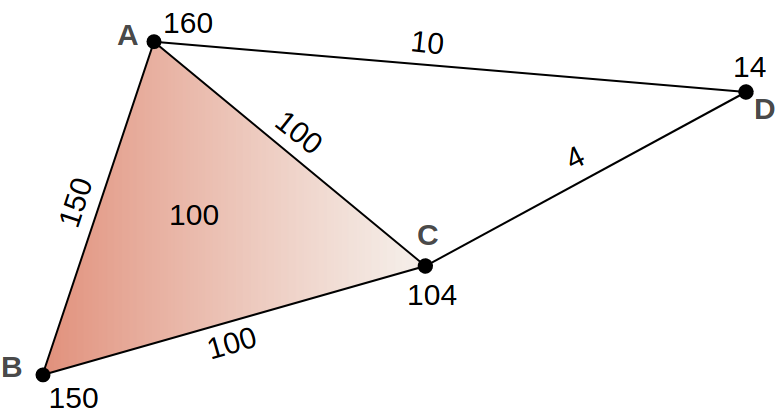
\includegraphics[height=2.3cm]{./figures/cc1.png}}%
\settowidth{\tempwidth}{\usebox{\tempbox}}%
\hfil\begin{minipage}[b]{\tempwidth}%
\raisebox{-\height}{\usebox{\tempbox}}%
\scriptsize{\captionof*{figure}{(b)}}%
\label{fig:co-authoship-complex}%
\end{minipage}%
\vspace{5pt}
%\end{table*}
\savebox{\tempbox}{\scriptsize{
\begin{blockarray}{cccccc}
\tiny{AB} & \tiny{AC} & \tiny{AD} & \tiny{BC} & \tiny{CD} \\
\begin{block}{(ccccc)c}
  3 & 0 & 1 & 0 & 0 & \tiny{AB} \\
  0 & 3 & 1 & 0 & -1 & \tiny{AC} \\
  1 & 1 & 2 & 0 & 1 & \tiny{AD} \\
  0 & 0 & 0 & 3 & -1 & \tiny{BC}\\
  0 & -1 & 1 & -1 & 2 & \tiny{CD}\\
\end{block}
\end{blockarray}}}%
\settowidth{\tempwidth}{\usebox{\tempbox}}%
\hfil\begin{minipage}[b]{\tempwidth}%
\raisebox{-\height}{\usebox{\tempbox}}%
\scriptsize{\captionof*{figure}{(c)}}%
\end{minipage}%
%\end{table*}
\caption{Constructing a simplicial complex from data. (a) Coauthorship data. (b) Coauthorship complex with corresponding cochains built from the data. (c) Degree-$1$ Laplacian of the coauthorship complex.}\label{fig:data2complex}
\end{figure}

\paragraph{Simplicial Laplacians.}
We are in this paper concerned with finite abstract simplicial complexes, although our method is applicable to a much broader setting, e.g.\ CW-complexes. In analogy with Hodge--de Rham theory~\cite{madsen1997calculus}, we then define the \emph{degree-$i$ simplicial Laplacian} of a simplicial complex $K$ as the linear map $\lap_i:C^i(K)\to C^i(K)$ specified by
\begin{equation*}
  \lap_i = \lapu_i + \lapd_i = \delta^{i\ast}\circ\delta^{i} + \delta^{i-1}\circ\delta^{i-1\ast},
\end{equation*}

where $\delta^{i\ast}$ is the adjoint of the coboundary with respect to the inner product (typically the one making the indicator function basis orthonormal). In most practical applications, the coboundary can be represented as a sparse matrix $B_i$ and the Laplacians can be efficiently computed as $L_i=B_i\transpose B_{i}+B_{i-1}B_{i-1}\transpose$. The matrices $B_0$ and $L_0$ are the classic graph incidence matrix and Laplacian.

Note that the Laplacians carry valuable topological information about the simplicial complex. In particular, the kernel of the $k$-Laplacian is isomorphic to the $k$-(co)homology of its associated simplicial complex~\cite{eckmann1944,horak2013spectra}.\footnote{In other words, the number of zero-eigenvalues tells us the number of $k$-dimensional holes.}
